\subsection{Total Sales Made}
This metric calculates the total number of sales that have been made within each product category..
\begin{lstlisting}[language=SQL]
SELECT 
    categoryname, 
    count(*) as count_sales_made
FROM sales_empl_view
GROUP BY categoryname
UNION ALL 
SELECT 
    'All Categories', 
    count(*) as count_sales_made
FROM sales_empl_view
ORDER BY categoryname
\end{lstlisting}
\textbf{Output Preview:}
\begin{center}
    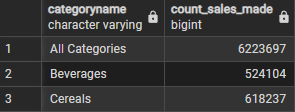
\includegraphics[width=0.6\linewidth]{Images/3.KPI_total-sales-made.png}
\end{center}
